\documentclass[11pt,a4paper]{article}

% packages
\usepackage[utf8]{inputenc}
\usepackage{amsmath}
\usepackage[T1]{fontenc}
\usepackage{setspace}
\usepackage{enumitem}
\usepackage{amsmath}
\usepackage{booktabs}
\usepackage{fullpage} 
\usepackage{tabularx}
\usepackage{amssymb, amstext, amsmath}
\usepackage{fancyhdr}
\usepackage{graphicx}
\usepackage{algorithmic}
\usepackage[ruled,vlined]{algorithm2e}
\usepackage{url}
\usepackage[bookmarks,unicode=true,pdftex,a4paper]{hyperref}
\usepackage[round]{natbib}
\usepackage[usenames,dvipsnames]{color, xcolor}
\headsep1cm

% macros
% misc
\newcommand\todo[1]{\textcolor{red}{TODO: #1}}
\newcommand\hide[1]{\textcolor{white}{#1}}

% formatting
\newcommand\bld[1]{\textbf{#1}}
\newcommand\ul[1]{\underline{#1}}
\newcommand\n[1]{\numprint{#1}}
\newcommand{\ts}{\textsuperscript}
\newcommand\red[1]{\textcolor{red}{#1}}
\newcommand\blue[1]{\textcolor{blue}{#1}}
\newcommand\link[2]{\href{#1}{\textcolor{blue}{\underline{#2}}}}

% sets
\newcommand\set[1]{\mathcal{#1}}
\newcommand\bb[1]{\mathbb{#1}}
\renewcommand\:{\colon} % for use with \sset, etc.
\newcommand{\sset}[1]{\left\{\,#1\,\right\}} % { ? }, automatic brackets
\newcommand{\ssets}[1]{\left\{#1\right\}} % {?}, automatic brackets
\newcommand{\ssetn}[1]{\{\,#1\,\}} % { ? }, normal brackets

% table formatting
% To better align bold entries in S columns (still broken)
% \usepackage{siunitx}
% \robustify\bfseries
% \newrobustcmd{\bfcell}{\bfseries}

% vector variables (taken from macros by Rainer Gemulla)
\newcommand\vect[1]{{\boldsymbol{#1}}}
\newcommand\va{\vect{a}}
\newcommand\vb{\vect{b}}
\newcommand\vc{\vect{c}}
\newcommand\vd{\vect{d}}
\newcommand\ve{\vect{e}}
\newcommand\vf{\vect{f}}
\newcommand\vg{\vect{g}}
\newcommand\vh{\vect{h}}
\newcommand\vi{\vect{i}}
\newcommand\vj{\vect{j}}
\newcommand\vk{\vect{k}}
\newcommand\vl{\vect{l}}
\newcommand\vm{\vect{m}}
\newcommand\vn{\vect{n}}
\newcommand\vo{\vect{o}}
\newcommand\vp{\vect{p}}
\newcommand\vq{\vect{q}}
\newcommand\vr{\vect{r}}
\newcommand\vs{\vect{s}}
\newcommand\vt{\vect{t}}
\newcommand\vu{\vect{u}}
\newcommand\vv{\vect{v}}
\newcommand\vw{\vect{w}}
\newcommand\vx{\vect{x}}
\newcommand\vy{\vect{y}}
\newcommand\vz{\vect{z}}
\newcommand\vzero{\vect{0}}
\newcommand\vone{\vect{1}}

\newcommand\valpha{\vect{\alpha}}
\newcommand\vbeta{\vect{\beta}}
\newcommand\veps{\vect{\epsilon}}
\newcommand\vdelta{\vect{\delta}}
\newcommand\vtheta{\vect{\theta}}
\newcommand\vsigma{\vect{\sigma}}
\newcommand\vpi{\vect{\pi}}
\newcommand\vlambda{\vect{\lambda}}

% matrix variables (taken from macros by Rainer Gemulla)
\newcommand\mA{\vect{A}}
\newcommand\mB{\vect{B}}
\newcommand\mC{\vect{C}}
\newcommand\mD{\vect{D}}
\newcommand\mE{\vect{E}}
\newcommand\mF{\vect{F}}
\newcommand\mG{\vect{G}}
\newcommand\mH{\vect{H}}
\newcommand\mI{\vect{I}}
\newcommand\mJ{\vect{J}}
\newcommand\mK{\vect{K}}
\newcommand\mL{\vect{L}}
\newcommand\mM{\vect{M}}
\newcommand\mN{\vect{N}}
\newcommand\mO{\vect{O}}
\newcommand\mP{\vect{P}}
\newcommand\mQ{\vect{Q}}
\newcommand\mR{\vect{R}}
\newcommand\mS{\vect{S}}
\newcommand\mT{\vect{T}}
\newcommand\mU{\vect{U}}
\newcommand\mV{\vect{V}}
\newcommand\mW{\vect{W}}
\newcommand\mX{\vect{X}}
\newcommand\mY{\vect{Y}}
\newcommand\mZ{\vect{Z}}
\newcommand\mzero{\vect{0}}

\newcommand{\mPi}{{\ensuremath{\vect{\Pi}}}}
\newcommand{\mSigma}{{\ensuremath{\vect{\Sigma}}}}
\newcommand{\mLambda}{{\ensuremath{\vect{\Lambda}}}}

% argmin, argmax
\DeclareMathOperator*{\argmin}{argmin} % amsmath package required
\DeclareMathOperator*{\argmax}{argmax} % amsmath package required

% matrix operations
\newcommand\xdiag{\operatorname{diag}}      
\newcommand\diag[1]{\xdiag\left(#1\right)}    % diagonal matrix


% new commands
\newcommand\op[1]{\operatorname{#1}}

% header and footer
\lhead{Advanced Methods in Text Analytics, FSS 2025}
\chead{}
\rhead{\thepage\ }
\cfoot{}
\pagestyle{fancy}

\title{Advanced Methods in Text Analytics \\ 
Exercise 6: Transformers - Part 2\\
\textbf{Solutions}}
\author{Daniel Ruffinelli}
\date{FSS 2025}

\begin{document}
\maketitle

\section{The Residual Stream}

\begin{enumerate}[label=(\alph*)]
    \item We have:
          \begin{align}
              \op{SA}(\mX) & = \op{softmax}\left(\frac{\mX\mW^Q(\mX\mW^K)^T}{\sqrt{d}}\right)\mX\mW^V
          \end{align}
          where the softmax function is applied row-wise and $\mX\mW^Q = \mQ$ is
          referred to as the query matrix, $\mX\mW^K = \mK$ is the key matrix, and
          $\mX\mW^V = \mV$ the value matrix.
          Recall that the factor $\frac{1}{\sqrt{d}}$ is used for numerical
          stability (scaled dot-product attention).
    \item We have:
          \begin{align}
              \op{FNN}(\mX) & = \text{ReLU}\left((\mX\mW_1 + \vb_1)\right)\mW_2 + \vb_2
          \end{align}
          where parameters are $\mW_1\in\bb{R}^{d\times m}$, $\vb_1\in\bb{R}^m$,
          $\mW_2\in\bb{R}^{m\times d}$, and $\vb_2\in\bb{R}^d$.
    \item We do this in stages. First, we focus on $\op{SA}$, its
          corresponding residual connection and layer normalization $\op{LN_1}$.
          We have:
          \begin{align}
              \op{\mO_1} & = \op{LN_1}(\op{SA}(\mX) + \mX)
          \end{align}
          Then, we focus on $\op{FNN}$, its corresponding residual connection
          and layer normalization area applied.
          That is:
          \begin{align}
              \op{\mO_2} & = \op{LN_2}(\op{FNN}(\mO_1) + \mO_1)
          \end{align}
          All together, we have:
          \begin{align}
              \op{TF}(\mX) & = \op{LN_2}(\op{FNN}(\op{LN_1}(\op{SA}(\mX) + \mX)) + \op{LN_1}(\op{SA}(\mX) + \mX)).
          \end{align}
    \item Layer normalization is used to normalize the vectors it is given as
          input.
          Concretely, given a vector $\vx\in\bb{R}^d$, the layer normalization
          operation is given by:
          \begin{align}
              \op{LN}(\vx) & = \frac{\vx - \mu}{\sigma} \gamma + \beta
          \end{align}
          where $\gamma$ and $\beta$ are learned parameters.
          This operation can be seen as a form of data centering and is commonly
          used so keep training stable, sometimes at the cost of performance on
          some downtream tasks.
          It can be applied anywhere in a network, including anywhere in a
          transformer layer.
          In fact, a common variant is the \emph{pre-norm} transformer, which
          applies layer normalization \emph{before} each of $\op{SA}$ and
          $\op{FNN}$.
          Typically, this variant also includes a single final layer
          normalization operation applied only to the output of the last
          transformer layer.
    \item To update parameters $\theta_{SA}$ of $\op{SA}$ w.r.t. some loss
          function $L$ during training, we need:
          \begin{align}\label{eq:weight_gradient}
              \frac{\partial L}{\partial \theta_{SA}} = \frac{\partial L}{\partial \op{SA}(\mH)}\frac{\partial \op{SA}(\mH)}{\partial \theta_{SA}},
          \end{align}
          where $\mH$ is the input to $\op{SA}$, which in turn is the output of
          the previous transformer layer $\op{TF_{i-1}}$.
          The term $\frac{\partial L}{\partial \op{SA}(\mH)}$ is the partial
          gradient received during backpropagation from the upper layer, the
          $\op{FNN}$ operator in the context of a transformer layer.
    \item Just as we received a gradient from the upper layer during training,
          we pass down the following gradient to the lower transformer layer
          $\op{TF_{i-1}}$ during backpropagation:
          \begin{align}\label{eq:input_gradient}
              \frac{\partial L}{\partial \mH} = \frac{\partial L}{\partial \op{SA}(\mH)}\frac{\partial \op{SA}(\mH)}{\partial \mH}.
          \end{align}
          This is the gradient of the output of $\op{TF_{i-1}}$ w.r.t. $L$, and
          is needed to compute the weight updates of the operators in lower
          layers that contribute to the computation of the input to $\op{TF_i}$,
          i.e.\ $\mH$.
    \item Let $\mO_1$ be the output of $\op{SA}$ with a residual connection
          around it, i.e.\ $\mO_1 = \op{SA}(\mH) + \mH$.
          Then, the gradient ``received'' from the upper layer is
          $\frac{\partial L}{\partial \mO_1}$.
          Eq.~\ref{eq:input_gradient} can then be rewritten as follows:
          \begin{align*}
              \frac{\partial L}{\partial \mH} & = \frac{\partial L}{\partial \mO_1}\frac{\partial \mO_1}{\partial \mH}                                                         \\
                                              & = \frac{\partial L}{\partial \mO_1}\frac{\partial (\op{SA}(\mH) + \mH)}{\partial \mH}                                          \\
                                              & = \frac{\partial L}{\partial \mO_1}\left(\frac{\partial \op{SA}(\mH)}{\partial \mH} + \frac{\partial \mH}{\partial \mH}\right) \\
                                              & = \frac{\partial L}{\partial \mO_1}\frac{\partial \op{SA}(\mH)}{\partial \mH} + \frac{\partial L}{\partial \mO_1}.
          \end{align*}
          In other words, when using residual connections, the gradient
          $\frac{\partial L}{\partial \mO_1}$ we receive from higher layers
          during backpropagation is passed down to lower layers by making a
          modification via the addition operation.

          Note that without the residual connection, the gradient we pass down
          would be modified by the multiplying factor
          $\frac{\partial \op{SA}(\mH)}{\partial \mH}$, and the additive term
          would not exist.
          Since such a multiplying factor can quickly reduce the size of the
          gradient that is passed backward during training, the residual
          connection was designed by
          \href{https://arxiv.org/abs/1512.03385}{\underline{He et al. 2015}} so
          that gradients can be more safely passed through an operator without
          it having a severe impact on those gradients.

          The name ``residual'' connection comes from the fact that, due to this
          change to prevent gradients from vanishing during training, the
          function $f(\mX) = \op{OP}(\mX)$ computed by some operator becomes
          $f(\mX) = \op{OP}(\mX) + \mX$.
          This means that we are learning to apply a suitable \emph{difference}
          $\op{OP}(\mX)$ that is added to given input $\mX$.
          In the context of a transformer layer, $\mX$ is a set of
          contextualized representations, so what each transformer layer learns
          is to add something to it \emph{if needed}.
          If $\mX$ is already suitable for the task, then a layer may make small
          modifications to it.
          This suggests that the main flow of information is coming from $\mX$,
          and not from $\op{OP}(\mX)$, or in other words, from the residual
          connections and not from the transformer layers.
          This perspective is known as the ``residual stream'' view of
          transformers, illustrated in the image below from Jurasfky and Martin
          (2024), Section 10.4.
          For evidence of the internal mechanisms of transformers being well 
          described by this perspective, see 
          \href{https://www.lesswrong.com/posts/AcKRB8wDpdaN6v6ru/interpreting-gpt-the-logit-lens}{here} 
          and \href{https://aclanthology.org/2022.emnlp-main.3/}{here}.
\end{enumerate}
\begin{center}
    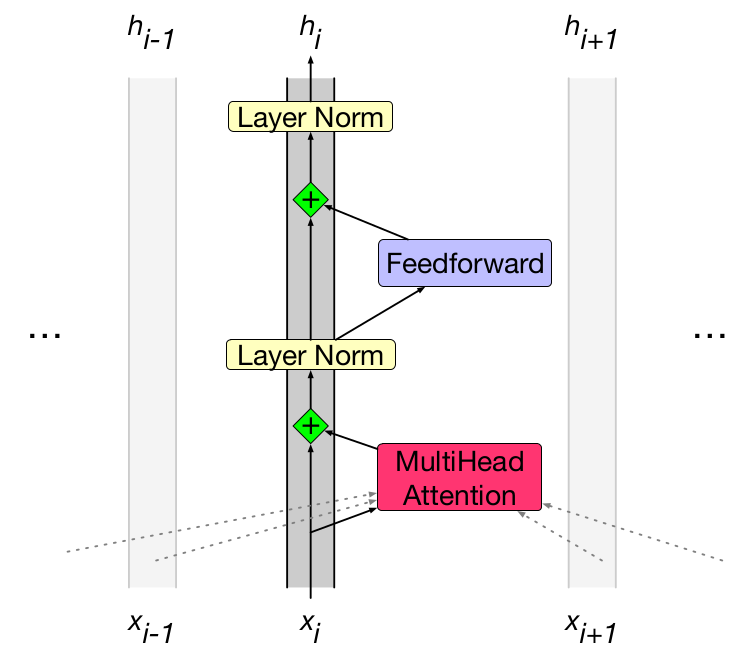
\includegraphics[scale=0.3]{img/residual_stream.png}
    \\ The Residual Stream. Information flows through residual connections.
\end{center}

\section{Attention Heads are Independent and Additive}

\begin{enumerate}[label=(\alph*)]
    \item We have:
          \begin{align}
              \op{MHA}(\mX) & = \left(SA_1(\mX) \oplus SA_2(\mX) \oplus \ldots \oplus SA_k(\mX)\right)\mW^O + \mX,
          \end{align}
          where $\oplus$ is the concatenation operator,
          $\mW_O\in\bb{R}^{kd\times d}$ is a parameter matrix that projects the
          concatenated vector back to $d$-dimensional residual space, and the
          additive term is the residual connection around MHA.
          Note that the size of $\mW^O$ is, indirectly, a design choice, as it
          depends on the number of attention heads (in this case k) and the size
          of tokens (in this case $d$).
    \item The operation in question here is the projection to residual space
          done by $\mW^O$.
          To see how this is parallelizable w.r.t.\ each
          $\op{SA}_i(\mX)$, let $\mO^i\in\bb{R}^{n\times d}$ be the output of
          $\op{SA_i}$, as described. After concatenating the output of each
          attention head, we have $\mO\in\bb{R}^{n\times kd}$ where $k$ is the
          number of attention heads. That is, we have the following block
          matrix:
          \begin{align}
              \mO & = \left[\mO^1 \mO^2 \ldots \mO^k\right].
          \end{align}
          Now, note that when computing each element $ij$ of $\mO\mW^O$,
          i.e.\ $[\mO\mW^O]_{ij}$, we compute the following dot product:
          \begin{align}
              [\mO\mW^O]_{ij} & = \sum_{h=1}^{kd} \mO_{ih}\mW^O_{hj}.
          \end{align}
          We can rewrite this dot product to make use of the $\mO^i$ components
          of $\mO$ more explicitly, as follows:
          \begin{align}
              [\mO\mW^O]_{ij} & = \sum_{h=1}^{d} \mO_{ih}\mW^O_{hj} + \sum_{h=d+1}^{2d} \mO_{ih}\mW^O_{hj} + \ldots + \sum_{h=(k-1)d+1}^{kd} \mO_{ih}\mW^O_{hj}         \\
                              & = \sum_{h=1}^{d} \mO^1_{ih}\mW^{O_1}_{hj} + \sum_{h=1}^{d} \mO^2_{ih}\mW^{O_2}_{hj} + \ldots + \sum_{h=1}^{d} \mO^k_{ih}\mW^{O_k}_{hj},
          \end{align}
          where we now defined $\mW^{O_i}\in\bb{R}^{d\times d}$ as the $i$-th
          block of $\mW^O$ that corresponds to $\mO^i$.
          That is, we can also see $\mW^O$ as the following block matrix:
          \begin{align}
              \mW^O & = \left[\mW^{O_1} \mW^{O_2} \ldots \mW^{O_k}\right]^\top.
          \end{align}
    \item From the solution to the previous subtasks, it follows that we can
          represent the general operation of $\op{MHA}$ as:
          \begin{align}
              \op{MHA}(\mX) & = \left[\mO^1\mO^2\ldots\mO^k\right] \begin{bmatrix}
                                                                       \mW^{O_1} \\
                                                                       \mW^{O_2} \\
                                                                       \ldots    \\
                                                                       \mW^{O_k}
                                                                   \end{bmatrix}
              + \mX.
          \end{align}
          And being as this is a matrix multiplication of block matrices, we
          can write this as the following linear combination:
          \begin{align}
              \op{MHA}(\mX) & = \sum_{i=1}^{k} \mO^i\mW^{O_i} + \mX,
          \end{align}
          where $\mM^i = \mW^{O_i}$ as desired.

          This equivalence shows that the output of the multi-head attention
          layer $\op{MHA}$ can be expressed as a linear combination of the
          outputs of each attention head $\op{SA}_i(\mX)$, where the weights
          of that linear combination are learned by the layer.
          Thus, each (weighted) attention head contributes to the
          learned representations by \emph{independently adding} to the 
          representations in residual space. 
          Indeed, the field of interpretability has identified that certain 
          attention heads learn specific roles that completely differ from other
          attention heads.
          For more details, see \href{https://transformer-circuits.pub/2021/framework/index.html}{here}.
\end{enumerate}

\section{Language Models with Transformers}

\begin{enumerate}[label=(\alph*)]
    \item Storing models during or after training is important to later be
          able to use them, e.g.\ for inference, fine-tuning or to continue
          training.
          PyTorch models have a state dictionary (state\_dict) that is
          usually stored on disk in so-called \emph{checkpoint} files.
          It's important that these files contain all the necessary
          information so that we may later be able to use the model.
          \emph{register\_buffer} is used to define ``parameters'' of a model
          that need to be stored in its state\_dict, but that aren't actually
          parameters in the learning sense.
          That is, they are not changed during training.
          Since we are implementing a non-parameterized positional encoding,
          we register these embeddings as buffers, because we later need
          them for using the model.
    \item The answer is not straightforward.
          If we look at the class from PyTorch that we use, it's the
          $\op{TransformerEncoder}$ class.
          But, as we'll see later, we apply a mask to our attention scores,
          which have an impact on the type of model we are using, so we'll come
          back to this in the next few questions.
          In addition, the model does not have cross-attention (attention
          between decoder and the outputs of the encoder), so it is definitely
          not an encoder-decoder model either.

          The code does have a component called a decoder, but what is that
          exactly?
          It's a linear layer that projects down to a vector space the size of
          our vocabulary, so while common, this naming convention can be
          confusing, as this decoding step refers to decoding in the
          tokenization sense.
          This projection, in combination with a softmax, will be used to
          produce probabilities over our vocabulary in order to predict the next
          token (if we construct the training examples correctly).
          But why isn't the softmax function there then?
          Well, as in our previous coding exercise, we will use
          $\op{CrossEntropyLoss}$, which includes the softmax function, so we
          need our model to output logits.
    \item This function is used to construct an attention mask.
          Masking is the process by which we ``block'' some entries in a tensor.
          In this context, the forward pass of the $\op{TransformerEncoder}$
          takes a mask as input along side the input sequence.
          This mask is added to the matrix of attention \emph{scores} in the
          self-attention layer.
          If scores are \emph{-Inf}, their attention weight (via softmax) is
          zero.
          Entry $ij$ in this matrix can be seen as how much attention input
          token $i$ pays to $j$.
          Thus, the mask is a matrix with zeros in the lower triangular, and
          the rest \emph{-Inf}.
    \item Given the attention mask we use, as explained in the answer above,
          this is a causal language model.
          Note that the use of this \emph{causal mask}, in combination with the
          lack of cross-attention, means we have a decoder-only model, despite
          using a $\op{TransformerEncoder}$ class.
          It is common to implement such a CLM using $\op{TransformerEncoder}$.
    \item See Jupyter notebook.
    \item We get validation perplexity (PPL) of about 500, which is somewhat
          higher than with the RNN, which was about 400.
          Recall that PPL can be interpreted as proportional to the vocabulary
          size, which is about 30K.
          In addition, and as discussed in previous tutorials, it can be
          interpreted as the average \emph{branching factor}, i.e.\ the average
          number of possible next words after a given one.

          The PPL values from the RNN and this transformer are inded comparable,
          as both models are evaluated on the same task using the same
          validation data (it's virtually the same code base).
          As for resources, they are also comparable.
          The embedding size is the same as the one used by the RNN, and both
          use dropout with default values as the only form of regularization.
          It's therefore likely can this slighly lower performance is due to
          the stronger inductive bias in the transformer model, i.e.\ it's
          overfitting.
          It would be nice to try to use a transformer with lower number of
          attention heads, or lower number of layers.
          And indeed, such tests are important to do on validation data before
          deciding which model will be used on test data or real-world data.
          We look at this further in the next question.
    \item See Jupyter notebook for details.
          When training longer, for 20 epochs, we see the transformer achieving
          a PPL of about 400, i.e.\ it achieves the same performance achieved by
          the RNN in a single epoch.
          But when training the RNN for 20 epochs, it gets a PPL of about 350,
          so while smaller, there is still a performance gap in favor of the
          RNN.

          W.r.t.\ changing model depth, we get slightly lower performance with
          a single layer, and a marginal improvement with 3 layers.
          But when using 6 layers performance drops, suggesting overfitting.

          Finally, we could use a
          \href{https://machinelearningmastery.com/using-learning-rate-schedule-in-pytorch-training/}{\underline{learning rate scheduler}}
          to get an increase in performance, as the learning rate is often a
          crucial hyperparameter in deep learning models, so processes like a
          \href{https://www.baeldung.com/cs/learning-rate-warm-up}{\underline{learning rate warmup}}
          are common practice when training large language models.

          In general, the transformer does not quite achieve the performance of
          the RNN in our tests, but it's possible that with other modifications
          we can get our transformer to performn better, e.g.\ using smaller
          hidden sizes, a different number of attention heads, etc.
          In addition, note that model stability should ideally be checked.
          In other words, how large is the variance of PPL when training the
          same model multiple times?
          Running the models in these tests multiple times suggests they are not
          quite stable, so that it's indeed possible that the transformer and
          the RNN are indeed performing similarly when comparing the mean and
          variance of PPL over, say, 10 different runs of each model.
\end{enumerate}

\end{document}
